% Operator screen mock-up (design only). Every element is from proposal Section 5.3; values are placeholders.
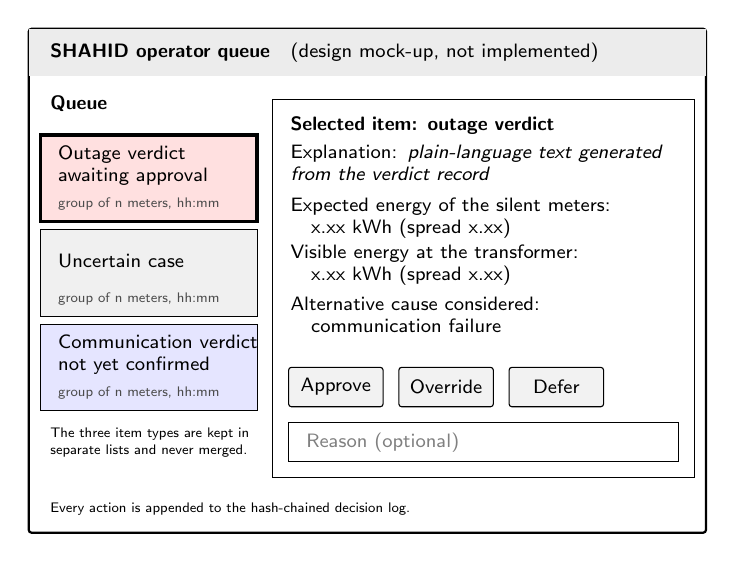
\begin{tikzpicture}[font=\scriptsize\sffamily, x=1mm, y=1mm]
\draw[rounded corners=1pt, thick] (0,0) rectangle (86,64);
\fill[gray!15] (0,58) rectangle (86,64);
\node[anchor=west] at (1.5,61) {\textbf{SHAHID operator queue}\quad (design mock-up, not implemented)};
% queue: three item types, never merged
\node[anchor=west] at (1.5,54.5) {\textbf{Queue}};
\foreach \y/\t/\c in {45/{Outage verdict\\awaiting approval}/red!12, 33/{Uncertain case}/gray!12,
                      21/{Communication verdict\\not yet confirmed}/blue!10} {
  \draw[fill=\c] (1.5,\y-5.5) rectangle (29,\y+5.5);
  \node[align=left, anchor=west] at (2.5,\y+1.6) {\t};
  \node[anchor=south west, font=\tiny\sffamily, gray!60!black] at (2.5,\y-5.3) {group of n meters, hh:mm};
}
\draw[very thick] (1.5,39.5) rectangle (29,50.5);
\node[anchor=north west, align=left, text width=26mm, font=\tiny\sffamily] at (1.5,14.5)
  {The three item types are kept in separate lists and never merged.};
% selected item
\draw (31,7) rectangle (84.5,55);
\node[anchor=north west, text width=51mm, align=left] at (32,54) {%
  \textbf{Selected item: outage verdict}\\[2pt]
  Explanation: \textit{plain-language text generated from the verdict record}\\[3pt]
  Expected energy of the silent meters:\\\quad x.xx kWh (spread x.xx)\\[1pt]
  Visible energy at the transformer:\\\quad x.xx kWh (spread x.xx)\\[3pt]
  Alternative cause considered:\\\quad communication failure};
% actions
\foreach \x/\t in {33/Approve, 47/Override, 61/Defer} {
  \draw[rounded corners=1pt, fill=gray!10] (\x,16) rectangle (\x+12,21);
  \node at (\x+6,18.5) {\t};
}
\draw (33,9) rectangle (82.5,14);
\node[anchor=west, text=gray] at (34,11.5) {Reason (optional)};
\node[anchor=west, font=\tiny\sffamily] at (1.5,3) {Every action is appended to the hash-chained decision log.};
\end{tikzpicture}
